% !TEX root=/home/tavant/these/manuscript/src/manuscript.tex

\section{Realistic heating and ionization}
  \label{sec-realistic_1D}
  In the study of \cref{{sec-1DPIC}}, the ionization and the heating mechanism are not physical, but allowed us to obtain a steady-state as in the simulations of \cref{ch-1}.

  Hence, we study the impact of the wall absorption in a case of self-consistent heating and ionization.
  The electrons are heated "inductively" with a radio-frequency (RF) electric field in the direction normal to the simulation grid \cite{meige2006a, lucken2018, turner1993}.
  The electrons are heated in the $y$ direction, and momentum is transferred to the $x$ and $z$ axis via electron-neutral collisions.
  The heating electric field $\vec{E_{rf}} = E_{rf} \vec{e_y}$ is independent of $x$ in the simulation domain, its frequency is $13.56$\,MHz, and its amplitude is adjusted in order to obtain the desired absorbed power $P_{abs} = < \vec{J_e} \cdot  \vec{E_{rf}}>$.
  


  \begin{table}[!htbp]
    \centering
    \begin{tabular}{@{} c | c | c}
      Parameter & value & unit \\ \hline
      Pressure & $0.1$ & mTorr\\
      $P_{abs}$ & $0.25$ & W/m$^{-3}$\\
      Length $L$&10&cm\\
    \end{tabular}
    \caption{Input parameters for the simulation using the self-consistent model.}
    \label{tab-PIC2}
  \end{table}

  \begin{figure}[!htbp]
    \center
    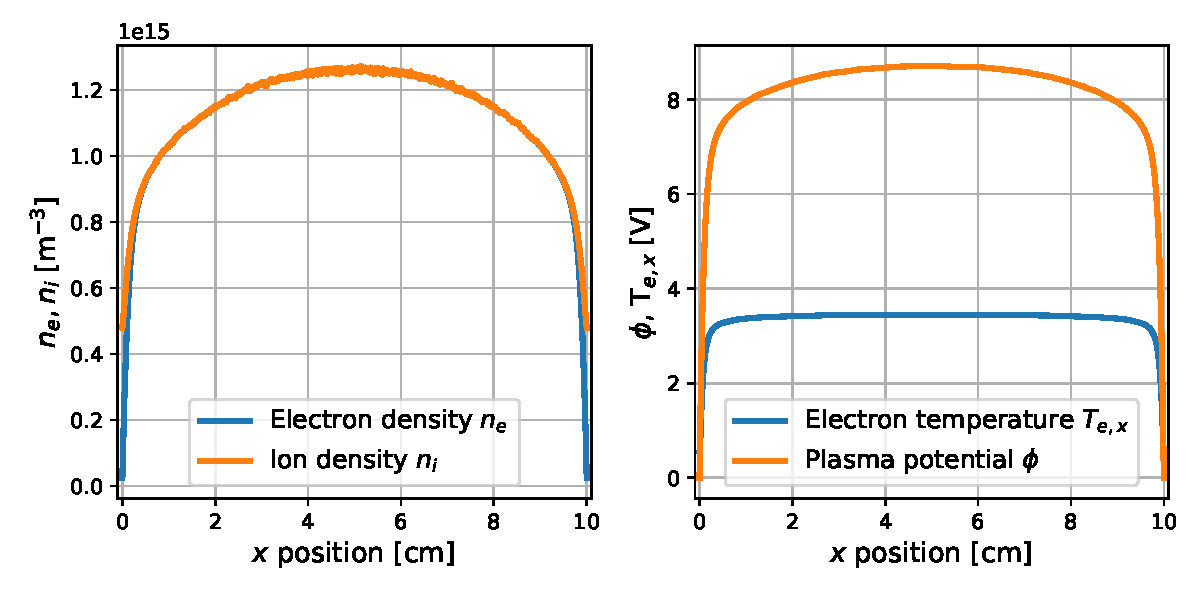
\includegraphics[width=0.9\textwidth]{ICP_results.pdf}
    \caption{Results of the PIC simulation for the self-consistent model, using RF inductive heating.}
    \label{fig-icpresults}
  \end{figure}

  \Cref{fig-icpresults} presents the simulation results for the electron density, plasma potential and electron temperature using the parameters of \Cref{tab-PIC2}.
  We can see that the different variables (density, electron temperature and the plasma potential) are not much affected compared to the results of \cref{sec-1DPIC}.

  \begin{figure}[!htbp]
    \centering
    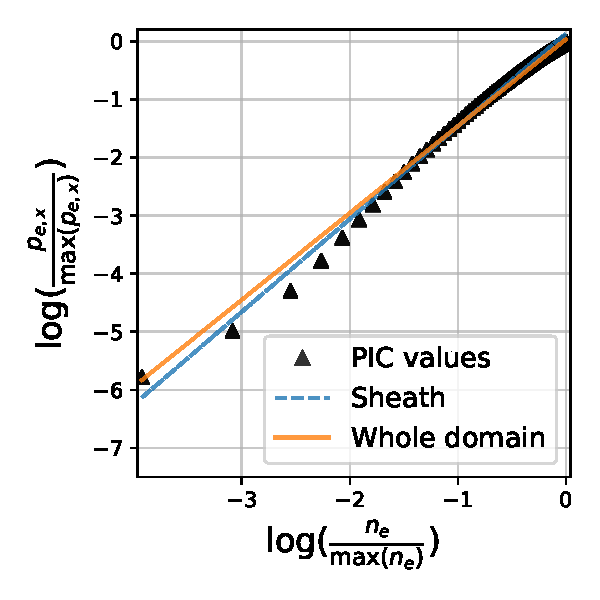
\includegraphics[width=\defaultwidth]{ICP_polyfit2.pdf}
    \caption{Estimation of the polytropic index in the sheath and in the whole domain in the PIC simulation using the self-consistent model.}
    \label{fig-icpfit}
  \end{figure}

  \Cref{fig-icpfit} presents the electron pressure as a function of the electron density measured in the simulation in log scale.
  We see that the trend is not purely linear. Hence, the linear regression used in order to obtain the polytropic index is conducted twice\string:
  \begin{itemize}
    \item In the whole domain\string: $\gamma=1.5$
    \item Only in the sheath\string: $\gamma=1.6$
  \end{itemize}
  The linear relation conducted of the whole domain is less precise than for the simulation result of \cref{sec-1DPIC} ($R^2=0.992$).
  However, we can see that the linear relation still describes quite well the electron evolution in the sheath.
  The polytropic indexes obtained with the self-consistent model are close to the simulation of \cref{sec-1DPIC} at the same pressure.

  \begin{figure}[!htbp]
    \centering
    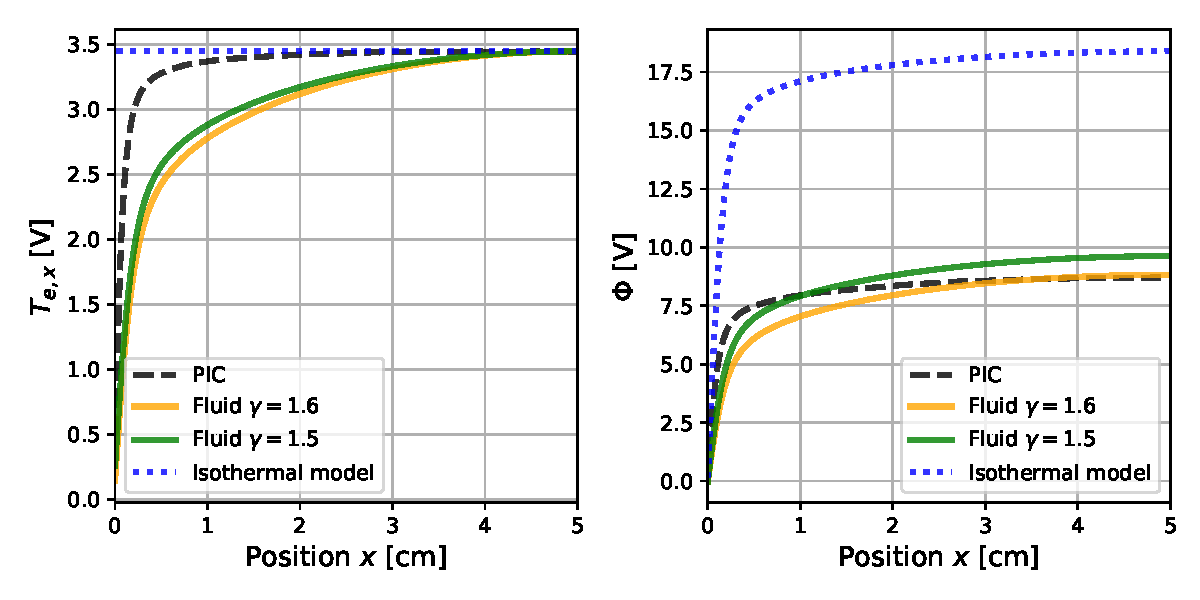
\includegraphics[width = 0.9\textwidth]{FluidComparisonICP.pdf}
    \caption{Comparison of the electron temperature and plasma potential measured in the PIC simulation with the prediction of the fluid model with $\gamma = 1.5$ (average index in the domain) and $\gamma=1.6$ (index in the sheath).}
    \label{fig-comp2}
  \end{figure}

  \Cref{fig-comp2} shows the comparison of the electron temperature and the plasma potential in the PIC simulation using the self-consistent model with the prediction of the fluid model of \cref{sec-fluid}.
  We can see that the agreement between the PIC results and the fluid models is less satisfactory than in \cref{fig-comp} when using the model unphysical plasma source, but it is still significantly better than the isothermal model.
  Hence, even with a self-consistent heating and ionization in the plasma, the polytropic model stands as a better model for the sheath and the pre-sheaths.
